% Mini research note on runtime, adjoints, and compute strategy.
\documentclass[11pt]{article}
% Shared preamble for the research-note series.
% Create note-specific content in the per-note directory; keep common macros here.
\usepackage[margin=1in]{geometry}
\usepackage[T1]{fontenc}
\usepackage[utf8]{inputenc}
\usepackage{amsmath,amssymb}
\usepackage{booktabs,longtable,array}
\usepackage{graphicx}
\usepackage{float}
\usepackage{enumitem}
\usepackage{xcolor}
\usepackage{hyperref}
\usepackage{caption}
\usepackage{titlesec}
\hypersetup{colorlinks=true, linkcolor=blue!60!black, urlcolor=blue!60!black, citecolor=blue!60!black}
\setlist[itemize]{leftmargin=1.25em, itemsep=0.2em, topsep=0.3em}
\setlist[enumerate]{leftmargin=1.4em, itemsep=0.2em, topsep=0.3em}
\setlength{\parindent}{0pt}
\setlength{\parskip}{0.6em}
\newcommand{\statusbox}[2]{%
  \noindent\fcolorbox{black}{gray!10}{%
    \parbox{\dimexpr\linewidth-2\fboxsep-2\fboxrule\relax}{%
      \textbf{Status:} #1\\#2
    }%
  }
}

% Shared notation helpers for the research-note series.
\newcommand{\Jlin}{J}
\newcommand{\Jphys}{J_{\mathrm{phys}}}
\newcommand{\Jsurf}{J_{\mathrm{surf}}}
\newcommand{\JdB}{J_{\mathrm{dB}}}
\newcommand{\phiopt}{\phi_{\mathrm{opt}}}
\newcommand{\sigmathreedb}{\sigma_{3\mathrm{dB}}}
\newcommand{\Nt}{N_t}
\newcommand{\Nphi}{N_{\phi}}
\newcommand{\Lfiber}{L}
\newcommand{\Pcont}{P}
\newcommand{\band}{\mathcal{B}_{\mathrm{Raman}}}
\newcommand{\todoitem}[1]{\textcolor{red!70!black}{\textbf{TODO:} #1}}


\title{Performance Model and Compute Strategy}
\author{Fiber Raman Suppression Project}
\date{Evidence snapshot: 2026-04-26}

\begin{document}
\maketitle

\begin{abstract}
This appendix explains how to think about runtime in the Raman-suppression
project. The main result is practical: for the canonical single-mode workload,
the fastest path is not ``turn on more threads inside one solve.'' The important
runtime decisions are to use adjoint gradients instead of finite differences,
keep FFTW internally single-threaded at the current grid sizes, and spend
parallel compute on independent runs such as sweeps, multistarts, and parameter
studies. The benchmark evidence is strong for the canonical single-mode case.
Multimode and long-fiber workloads should be remeasured before reusing the same
threading conclusions.
\end{abstract}

\section*{Claim Status}
\statusbox{established for the canonical single-mode workload}{The benchmark
data support a stable compute rule for the current SMF-28 single-mode problem:
use adjoint gradients, keep FFTW internal threading at one thread, and parallelize
across independent jobs when possible. The caveat is important: multimode and
long-fiber studies may move the bottleneck, so those directions should be
benchmarked separately before making infrastructure decisions.}

\section{Question and Thesis}

The question in this appendix is not whether the physics model is correct. It is
where compute effort actually helps.

The thesis is:
\[
    \text{adjoint gradients} + \text{task-level parallelism}
    \quad \text{beat} \quad
    \text{more internal threads for one canonical solve}.
\]

That matters because this project has several tempting but expensive paths:
full-grid gradients, multistart searches, reduced-basis ladders, second-order
diagnostics, multimode runs, and long-fiber runs. A bad performance model would
push effort toward the wrong machine or the wrong optimization method.

\subsection*{Intuition Check}

If one solve is mostly serial, adding more workers to that one solve does not
help much. The better use of workers is to run many independent solves at the
same time: different starts, different fiber settings, different basis sizes,
or different validation cases.

\section{The Cost Model}

The baseline objective is the output Raman-band energy fraction,
\[
    \Jphys(\phi)
    =
    \frac{\sum_{\omega_k\in\band}|u_{\omega_k}(L;\phi)|^2}
         {\sum_k |u_{\omega_k}(L;\phi)|^2},
\]
with optional regularization before the dB transform:
\[
    \Jsurf(\phi)
    =
    \Jphys(\phi)
    + \lambda_{\mathrm{gdd}}R_{\mathrm{gdd}}(\phi)
    + \lambda_{\mathrm{edge}}R_{\mathrm{edge}}(\phi),
    \qquad
    F(\phi)=10\log_{10}\Jsurf(\phi).
\]
The phase vector can have thousands of entries. In the canonical grid,
\(\Nt=8192\), so a naive central-difference gradient would cost roughly
\[
    2\Nt\,C_{\mathrm{fwd}}
    =
    16384\,C_{\mathrm{fwd}},
\]
where \(C_{\mathrm{fwd}}\) is the cost of one forward fiber solve. That is not a
reasonable inner loop for L-BFGS.

The adjoint method changes the scaling. One cost-and-gradient evaluation is
approximately
\[
    C_{\mathrm{grad}}
    \approx
    C_{\mathrm{fwd}} + C_{\mathrm{adj}} + C_{\mathrm{regularizer}},
\]
where \(C_{\mathrm{adj}}\) is the backward sensitivity solve. The important
point is that this cost does not grow like the number of phase pixels.

\begin{figure}[H]
\centering
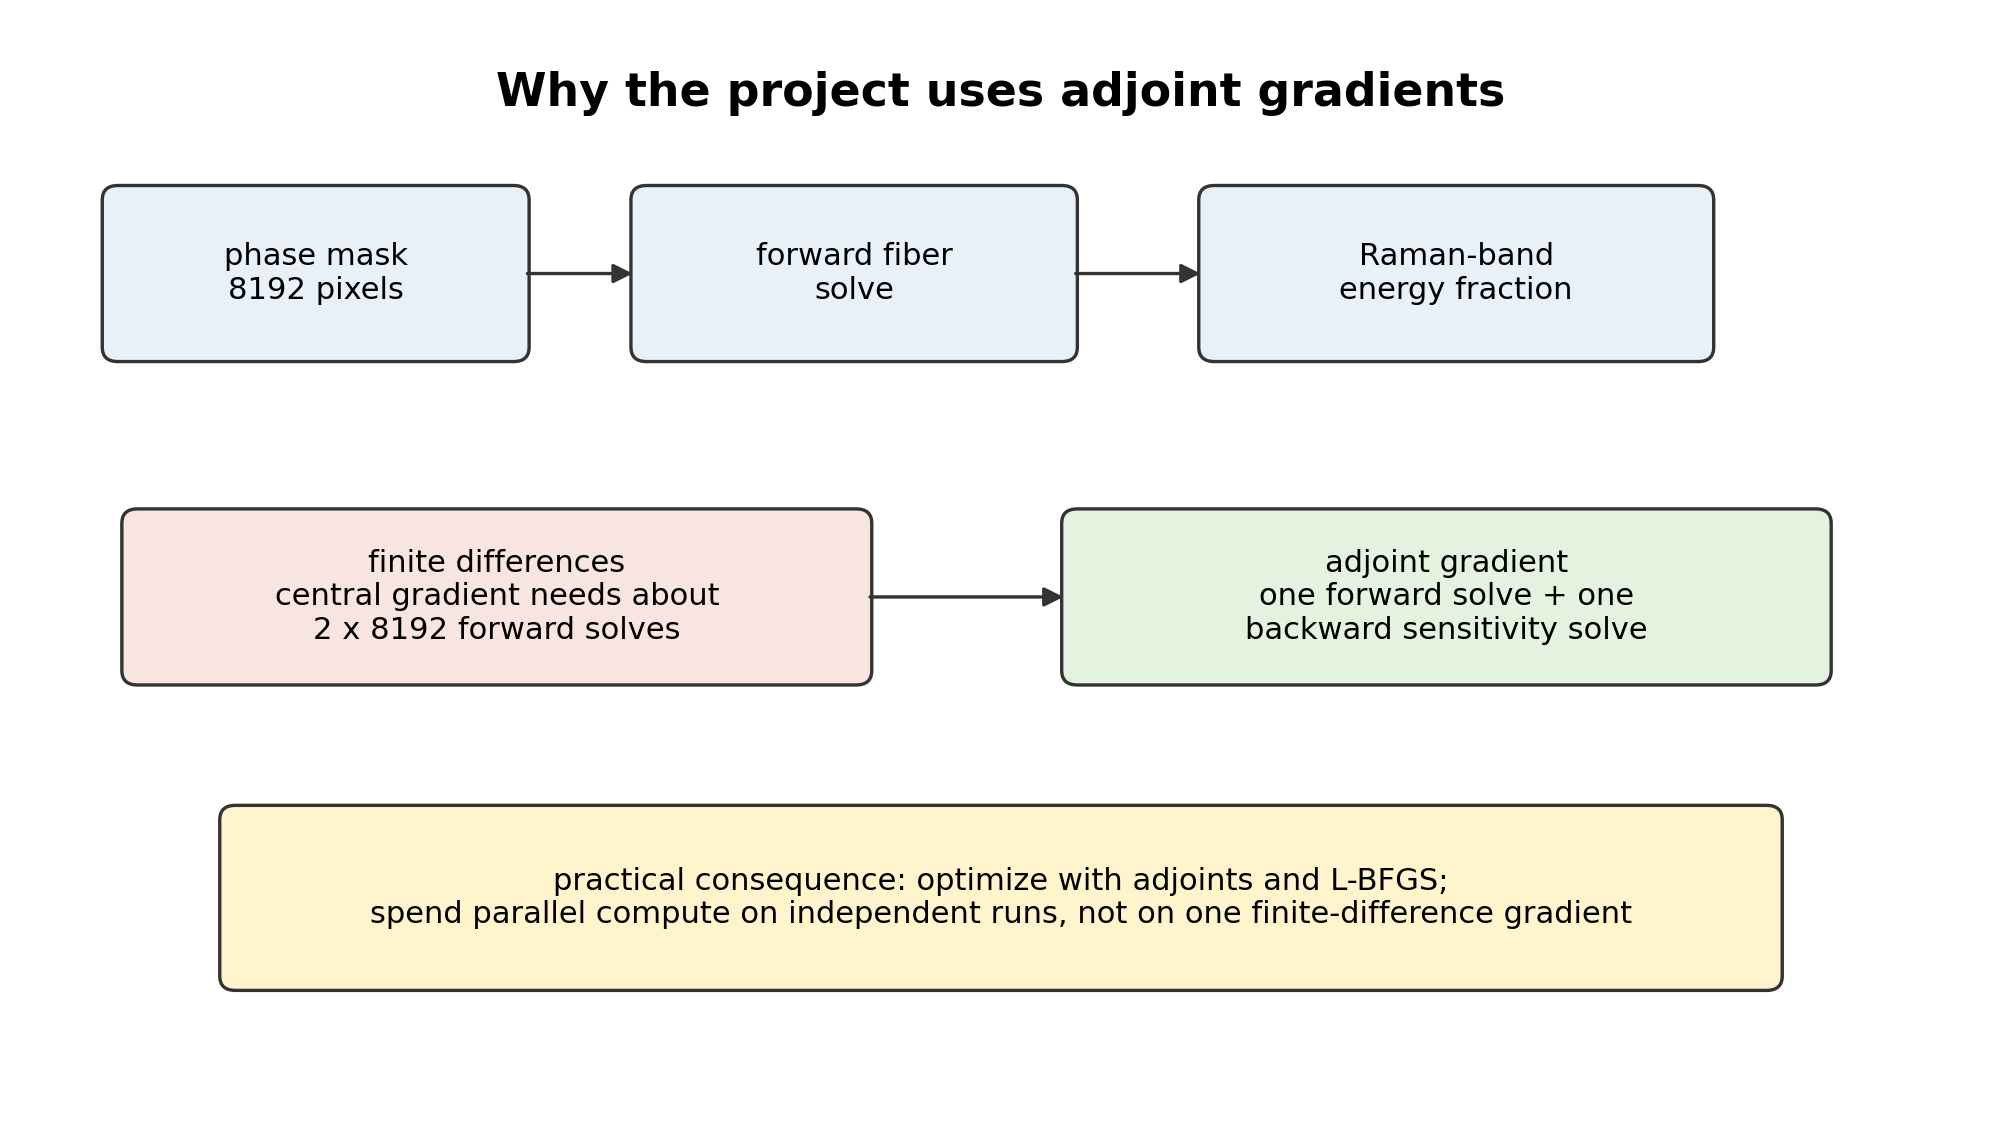
\includegraphics[width=0.96\linewidth]{figures/performance_cost_model.png}
\caption{Why adjoints are the default gradient method. Finite differences ask
one question per phase pixel. The adjoint solve gives the whole phase-gradient
direction in one backward sensitivity pass.}
\end{figure}

\subsection*{Intuition Check}

Finite differences are like changing every knob one at a time and rerunning the
whole experiment. The adjoint is like one backward calculation that tells us
which way all knobs should move.

\section{Measured Runtime Evidence}

The canonical benchmark used an SMF-28 single-mode setting with
\(L=2\,\mathrm{m}\), \(P=0.2\,\mathrm{W}\), \(\Nt=8192\), Julia 1.12.4, and an
Apple M3 Max host. The exact numbers should not be treated as universal
hardware constants. The shape of the result is the important part.

\begin{figure}[H]
\centering
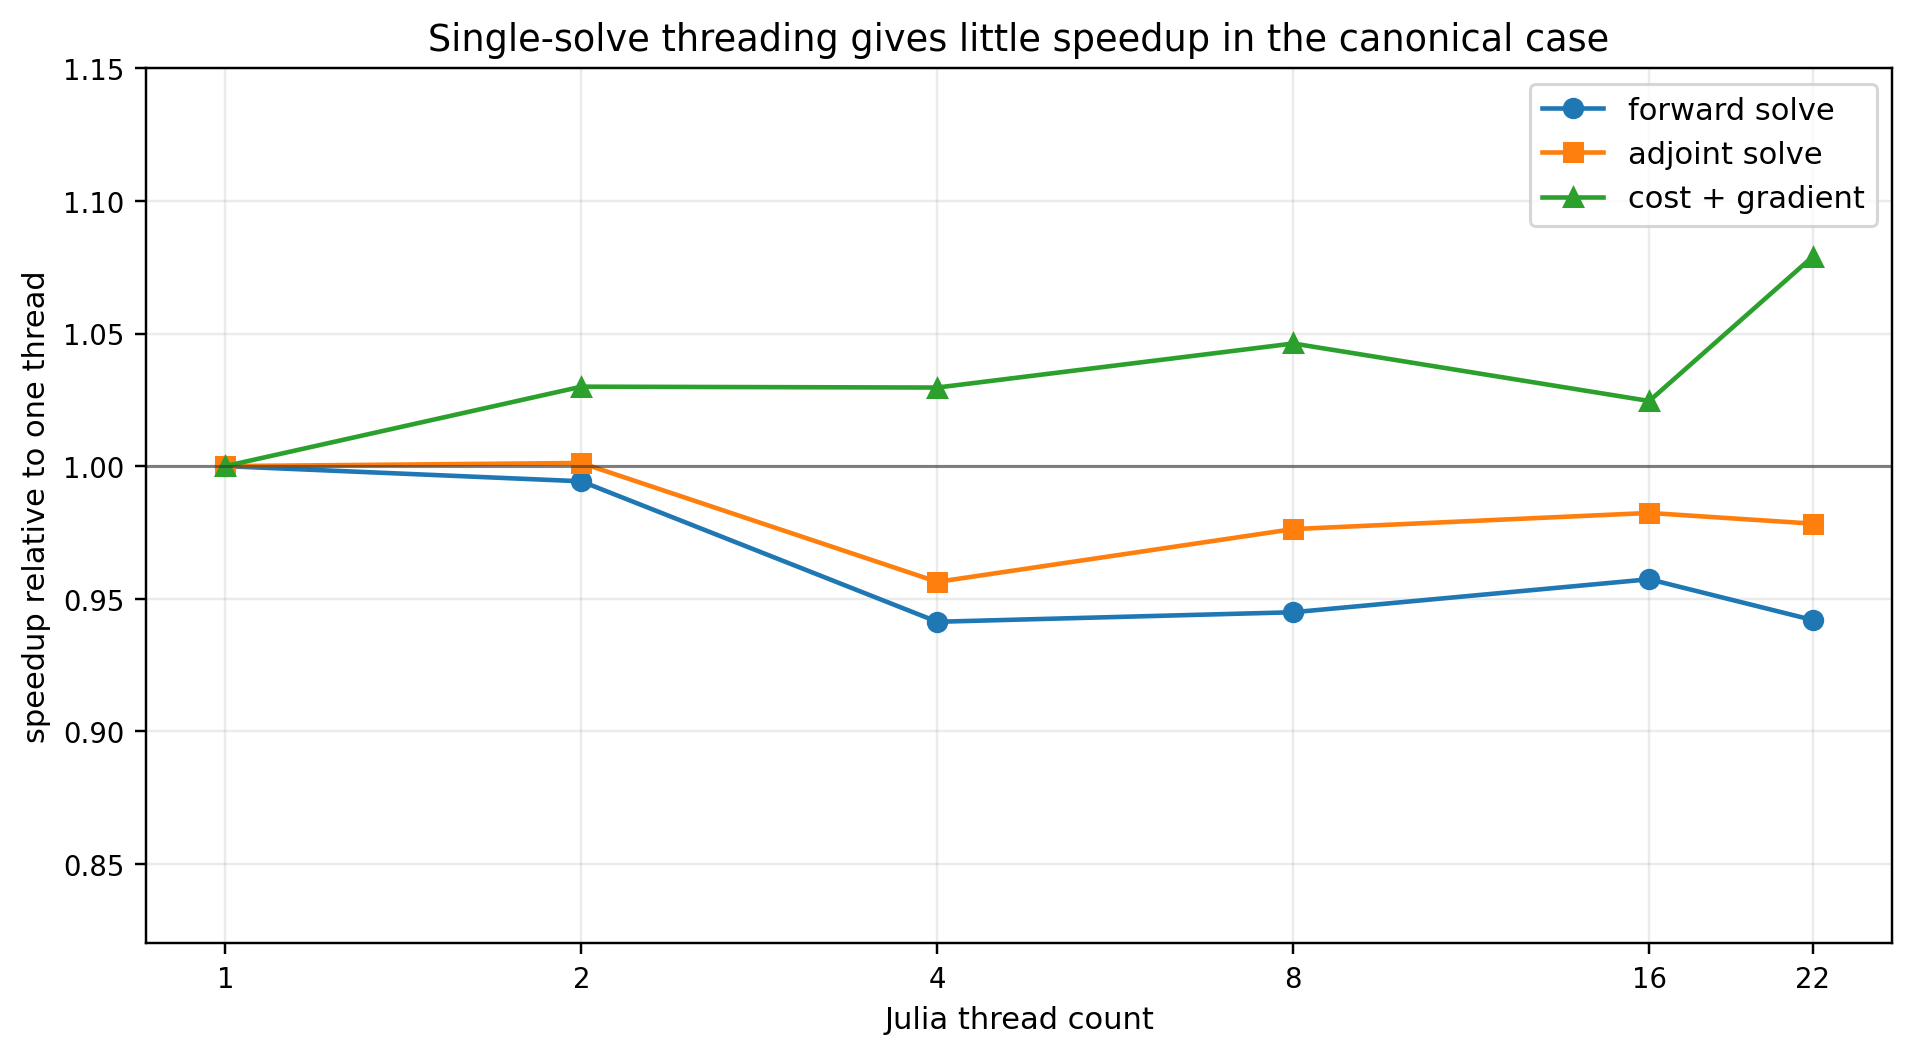
\includegraphics[width=0.90\linewidth]{figures/single_solve_thread_speedup.png}
\caption{Single-solve threading speedup relative to one Julia thread. Forward
and adjoint solves do not improve; the full cost-and-gradient call improves
only weakly. This is the measured reason the project does not treat internal
thread count as the main lever for the canonical single-mode workload.}
\end{figure}

\begin{center}
\small
\resizebox{\linewidth}{!}{%
\begin{tabular}{>{\raggedright\arraybackslash}p{0.24\linewidth}
                >{\raggedleft\arraybackslash}p{0.16\linewidth}
                >{\raggedleft\arraybackslash}p{0.18\linewidth}
                >{\raggedleft\arraybackslash}p{0.18\linewidth}
                >{\raggedright\arraybackslash}p{0.30\linewidth}}
\toprule
\textbf{Measured mode} & \textbf{One thread} & \textbf{Best observed} &
\textbf{Fitted ceiling} & \textbf{Takeaway} \\
\midrule
Forward solve & \(1.178\,\mathrm{s}\) & \(1.178\,\mathrm{s}\) &
\(1.00\times\) & Extra Julia threads do not speed up the forward solve. \\
Adjoint solve & \(1.325\,\mathrm{s}\) & \(1.323\,\mathrm{s}\) &
\(1.00\times\) & The measured difference is noise-level for planning. \\
Cost + gradient & \(2.708\,\mathrm{s}\) & \(2.510\,\mathrm{s}\) &
\(1.05\times\) & There is a small gain, but not enough to justify a large
single-job machine for this case. \\
\bottomrule
\end{tabular}}
\end{center}

The kernel-level timing tells the same story. The adjoint right-hand side is
materially heavier than the forward right-hand side, and the raw FFT timings do
not explain the whole runtime.

\begin{figure}[H]
\centering
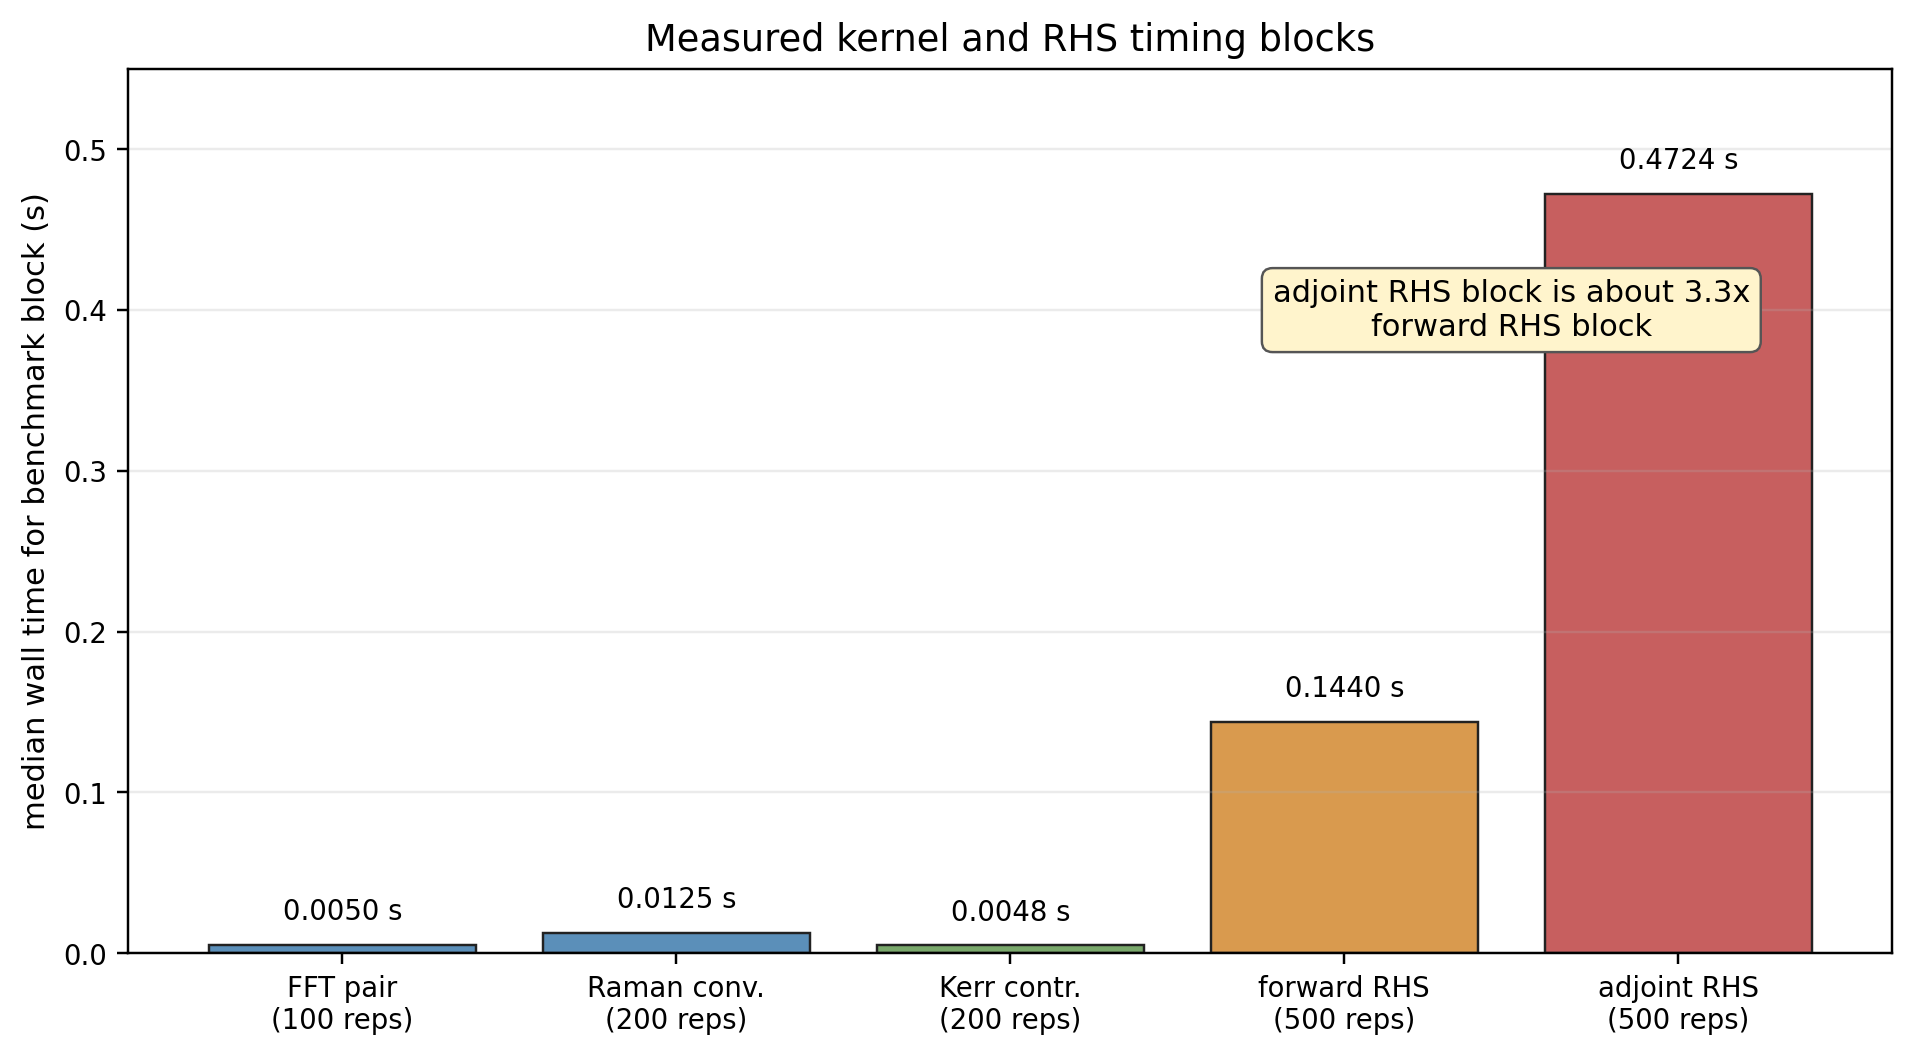
\includegraphics[width=0.92\linewidth]{figures/kernel_timing_summary.png}
\caption{Representative timing blocks from the benchmark artifact. The adjoint
right-hand-side block is about \(3.3\times\) the forward right-hand-side block,
so gradient evaluations are much more than ``one forward solve with a small
extra step.''}
\end{figure}

\begin{center}
\small
\resizebox{\linewidth}{!}{%
\begin{tabular}{>{\raggedright\arraybackslash}p{0.30\linewidth}
                >{\raggedleft\arraybackslash}p{0.16\linewidth}
                >{\raggedleft\arraybackslash}p{0.16\linewidth}
                >{\raggedright\arraybackslash}p{0.38\linewidth}}
\toprule
\textbf{Block} & \textbf{Repetitions} & \textbf{Median time} &
\textbf{Interpretation} \\
\midrule
FFT forward + inverse pair & 100 & \(0.0050\,\mathrm{s}\) &
Single-thread FFT planning is fast at this grid size. \\
Raman frequency convolution & 200 & \(0.0125\,\mathrm{s}\) &
Raman terms are visible but not the only cost. \\
Kerr tensor contraction & 200 & \(0.0048\,\mathrm{s}\) &
Trivial in this single-mode case; important again in multimode. \\
Forward RHS block & 500 & \(0.1440\,\mathrm{s}\) &
About \(288\,\mu\mathrm{s}\) per call. \\
Adjoint RHS block & 500 & \(0.4724\,\mathrm{s}\) &
About \(945\,\mu\mathrm{s}\) per call, partly due to forward-solution
interpolation inside the adjoint. \\
\bottomrule
\end{tabular}}
\end{center}

\subsection*{Intuition Check}

The adjoint is still the right method because it replaces thousands of forward
solves. But it is not free. When a note says ``one gradient evaluation,'' read
that as a forward solve plus a heavier backward sensitivity solve.

\section{Why FFTW Internal Threading Is Not the Lever}

At \(\Nt=8192\), internal FFTW threading is counterproductive in the benchmark.
The one-thread FFT pair block took \(0.0050\,\mathrm{s}\). The best multi-thread
FFT pair block took \(0.0822\,\mathrm{s}\), about a \(16.3\times\) slowdown for
that isolated FFT test.

The likely reason is overhead. The FFTs at this grid size are not large enough
to pay for the extra thread coordination inside each transform. This is why the
current rule is:
\[
    \texttt{FFTW.set\_num\_threads(1)}
    \quad \text{unless a new workload is remeasured.}
\]

There is also a reproducibility tradeoff. Deterministic FFT planning was
measured to be slower than timed plan selection, but the deterministic path
keeps independent optimizer runs comparable.

\begin{figure}[H]
\centering
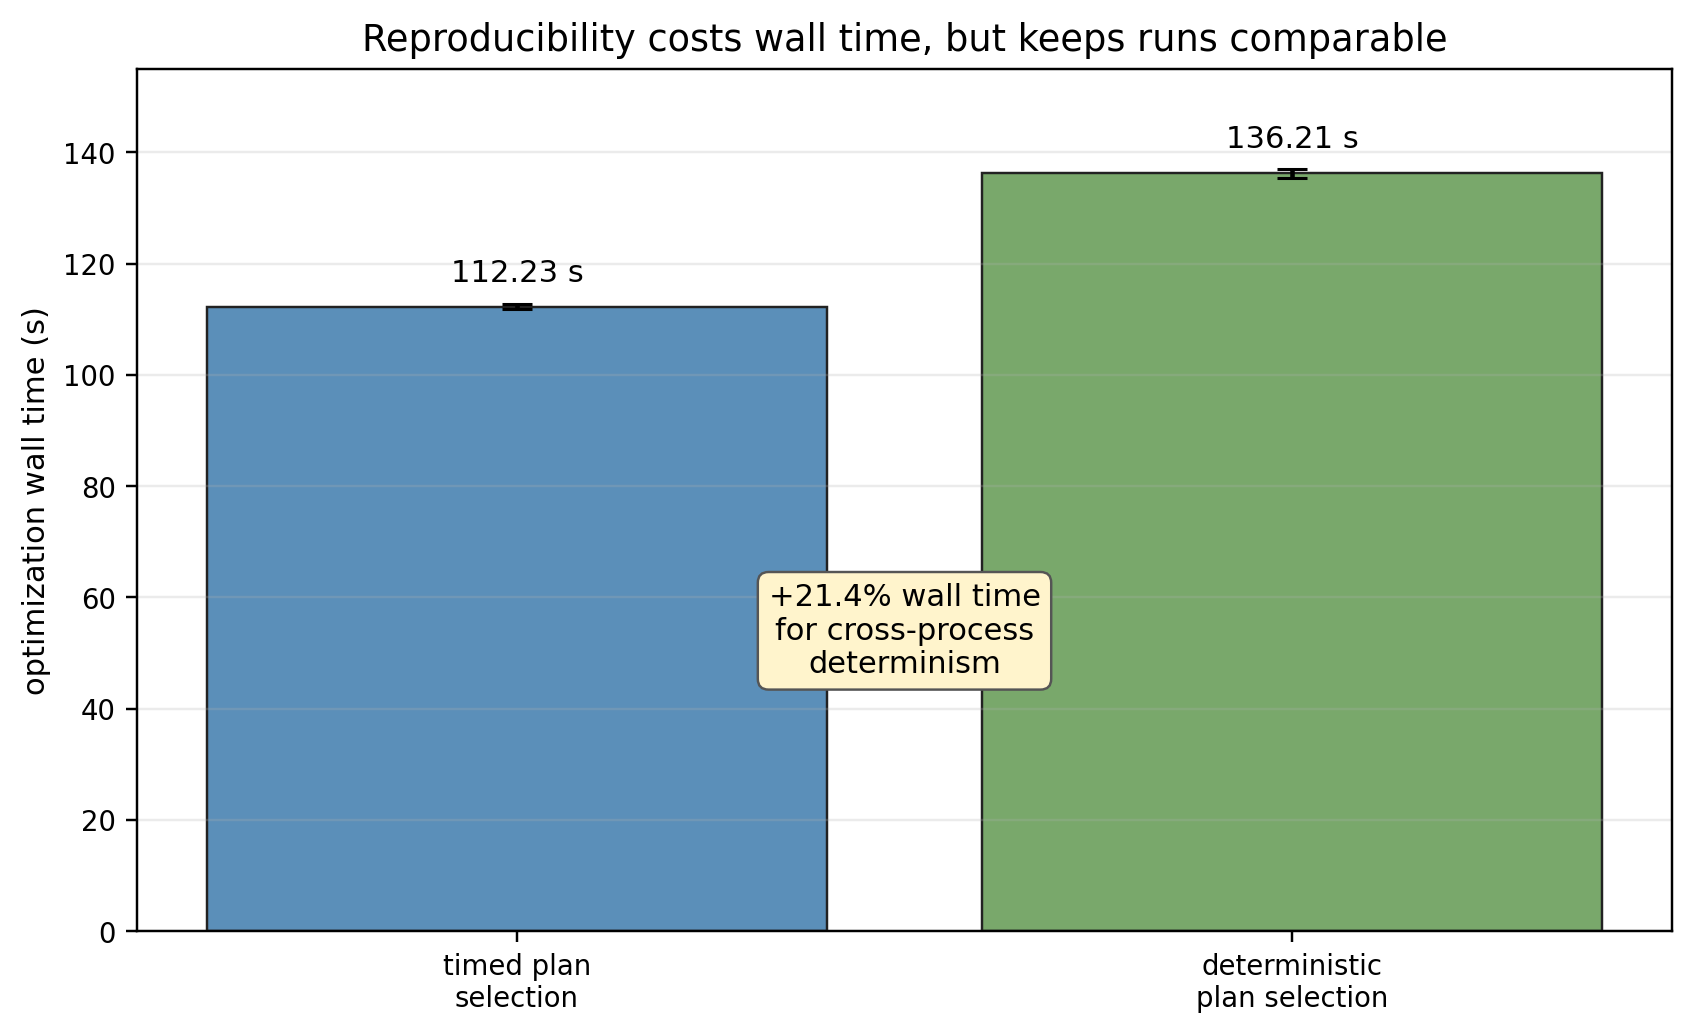
\includegraphics[width=0.78\linewidth]{figures/determinism_speed_tradeoff.png}
\caption{Deterministic FFT planning costs wall time in the benchmark, but it
removes a source of cross-process plan-selection variation. The measured
slowdown was \(21.4\%\), inside the project's accepted reproducibility budget.}
\end{figure}

\subsection*{Intuition Check}

There are two separate threading questions. Julia threads control how much
parallel work the program can schedule. FFTW threads control how many workers
FFTW uses inside one transform. For this grid, FFTW's internal threads make the
FFT block slower, not faster.

\section{Parallelism Strategy}

Amdahl's law says that if a fraction \(p\) of one job is parallelizable, then
the best possible strong-scaling speedup on \(N\) workers is
\[
    S_{\mathrm{Amdahl}}(N)
    =
    \frac{1}{(1-p)+p/N}.
\]
For the canonical single-mode benchmark, the fitted \(p\) values were
effectively zero for forward and adjoint solves, and about \(0.05\) for the
full cost-and-gradient call. That gives a speedup ceiling near \(1.0\times\),
or only about \(1.05\times\) for the full gradient call.

That does not mean parallel compute is useless. It means the better scaling
surface is weak scaling across independent jobs:
\[
    \text{many independent starts or sweep points}
    \quad \Rightarrow \quad
    \text{many cores can stay busy}.
\]

\begin{center}
\small
\begin{tabular}{>{\raggedright\arraybackslash}p{0.42\linewidth}
                >{\raggedright\arraybackslash}p{0.48\linewidth}}
\toprule
\textbf{Low-leverage use of cores} & \textbf{High-leverage use of cores} \\
\midrule
More internal FFTW threads for one canonical solve &
Many independent sweep points \\
Buying a large VM for one single-mode cost-and-gradient call &
Many multistart runs with separate random seeds \\
Assuming a multimode bottleneck from single-mode timings &
Remeasuring multimode kernels before choosing the machine \\
\bottomrule
\end{tabular}
\end{center}

\subsection*{Intuition Check}

One hard-to-parallelize job is like one checkout line with many idle cashiers.
Many independent runs are like opening many checkout lines at once.

\section{Compute Discipline}

The practical machine rule is:
\begin{itemize}
    \item local or orchestration hosts are appropriate for editing, plotting,
    PDF generation, indexing, and light checks;
    \item heavy simulation campaigns belong on the burst machine through the
    approved wrapper;
    \item Julia simulation runs should be launched with threading enabled, but
    FFTW internal threading should remain at one thread unless the workload has
    been remeasured;
    \item the burst machine is most useful for multimode studies, long sweeps,
    multistarts, and other embarrassingly parallel jobs;
    \item stop the burst machine when the heavy job is complete.
\end{itemize}

For the current canonical single-mode case, a large high-CPU VM is not justified
for one optimization run. It can still be justified if the job list contains
many independent runs.

\section{Multimode and Long-Fiber Caveat}

This appendix should not be read as ``performance is solved.'' It is a scoped
single-mode performance model.

For \(M=1\), FFT-heavy reasoning is often a decent first approximation. For
\(M\ge 3\), the Kerr tensor contractions and memory traffic can dominate the
right-hand side. Long-fiber runs may also change runtime through solver step
counts, stiffness, and output checkpointing. Those cases need their own timing
artifacts before making strong claims.

\subsection*{Intuition Check}

Changing from one mode to many modes is not just making the same calculation a
little bigger. It changes the shape of the work. The benchmark target has to
match the research target.

\section{Image Rule for This Appendix}

Most notes in this series pair phase diagnostics with spectral-evolution heat
maps. This appendix is different: it does not introduce a new optimized optical
field. Its figures are therefore benchmark diagrams and timing charts rather
than phase-profile pages. Optical-result notes should still include the paired
phase-diagnostic and heat-map pages.

\section{Presentation Capsule}

If this appendix becomes a compute-methods slide, the clean message is:
\begin{itemize}
    \item The adjoint is what makes full-grid optimization feasible; finite-differencing thousands of phase pixels is not practical.
    \item More threads inside one solve are not automatically the best speedup path; workload shape and run-level parallelism matter.
    \item Deterministic numerics can be worth a small runtime cost because optimizer comparisons need reproducible surfaces.
    \item This is a support slide: use it to explain how the research was run responsibly, not as a primary physics-result slide.
\end{itemize}

\section{Reproduction Capsule}

Benchmark commands should be run only when the machine and workload match the
question being asked:
\[
\texttt{julia -t auto --project=. scripts/research/benchmarks/benchmark\_threading.jl}
\]
\[
\texttt{julia -t auto --project=. scripts/workflows/run\_benchmarks.jl}
\]

For a new benchmark, record at least:
\begin{itemize}
    \item Julia version, host CPU, memory, Julia thread count, BLAS thread
    count, and FFTW thread count;
    \item fiber, length, power, grid size, number of modes, time window, and
    solver tolerances;
    \item forward solve timing, adjoint solve timing, full cost-and-gradient
    timing, and any isolated kernel timing used to justify a conclusion;
    \item whether the benchmark is single-mode, multimode, long-fiber, or a
    sweep/multistart workload.
\end{itemize}

\section{Key Lessons and Limitations}

\textbf{Use adjoints.} Full-grid finite differences are not viable for routine
optimization.

\textbf{Do not overbuy single-job threads.} The canonical single-mode
cost-and-gradient call has only a small measured strong-scaling gain.

\textbf{Keep deterministic numerics visible.} A slower deterministic FFT plan
can be the right choice if it keeps optimizer comparisons trustworthy.

\textbf{Parallelize the experiment list.} Sweeps, multistarts, basis ladders,
and validation batches are where parallel compute gives the cleanest return.

\textbf{Remeasure outside the canonical case.} Multimode and long-fiber studies
can have different bottlenecks, so their compute plans should be based on their
own benchmark artifacts.

\section{Sources and References}

\begin{thebibliography}{9}

\bibitem{frigo2005}
M. Frigo and S. G. Johnson.
``The design and implementation of FFTW3.''
\textit{Proceedings of the IEEE}, 93(2), 216--231, 2005.
\url{https://doi.org/10.1109/JPROC.2004.840301}

\bibitem{amdahl1967}
G. M. Amdahl.
``Validity of the single processor approach to achieving large scale computing
capabilities.''
\textit{AFIPS Conference Proceedings}, 30, 483--485, 1967.
\url{https://doi.org/10.1145/1465482.1465560}

\bibitem{gustafson1988}
J. L. Gustafson.
``Reevaluating Amdahl's law.''
\textit{Communications of the ACM}, 31(5), 532--533, 1988.
\url{https://doi.org/10.1145/42411.42415}

\bibitem{giles2000}
M. B. Giles and N. A. Pierce.
``An introduction to the adjoint approach to design.''
\textit{Flow, Turbulence and Combustion}, 65, 393--415, 2000.
\url{https://doi.org/10.1023/A:1011430410075}

\bibitem{griewank2008}
A. Griewank and A. Walther.
\textit{Evaluating Derivatives: Principles and Techniques of Algorithmic
Differentiation}, 2nd ed.
SIAM, 2008.
\url{https://doi.org/10.1137/1.9780898717761}

\bibitem{liu1989}
D. C. Liu and J. Nocedal.
``On the limited memory BFGS method for large scale optimization.''
\textit{Mathematical Programming}, 45, 503--528, 1989.
\url{https://doi.org/10.1007/BF01589116}

\bibitem{nocedal2006}
J. Nocedal and S. J. Wright.
\textit{Numerical Optimization}, 2nd ed.
Springer, 2006.
\url{https://doi.org/10.1007/978-0-387-40065-5}

\bibitem{agrawal2019}
G. P. Agrawal.
\textit{Nonlinear Fiber Optics}, 6th ed.
Academic Press, 2019.
\url{https://www.sciencedirect.com/book/9780128170427/nonlinear-fiber-optics}

\end{thebibliography}

\end{document}
